\documentclass[12pt]{article}
\usepackage{amsmath}
\usepackage{graphicx}
\usepackage{hyperref}
\usepackage[latin1]{inputenc}
\usepackage[top=2cm, bottom=2cm, left=2cm, right=2cm, headsep=14pt]{geometry}
\usepackage[T1]{fontenc}
\usepackage[utf8]{inputenc}

\title{Report 1}
\author{Group 2}
% \author[2]{Hoang Duc Minh, Le Tan Nhat Linh, Luong Hung Son,}
% \author[3]{ Nguyen Vu Hung, Truong Hai Long}
\date{January 17, 2018}

\begin{document}
\maketitle
  \section{Designing protocol}
    We used predefined message system to create handshaking. It helps to make sure that the connection and transmission between server and client is consistent. When the connection is established, the server will send a message, if the client verify the message then it will start to do the task and send information to the server. After that, the process starts again until the file is transferred.
    \begin{figure}[h]
        \centering
       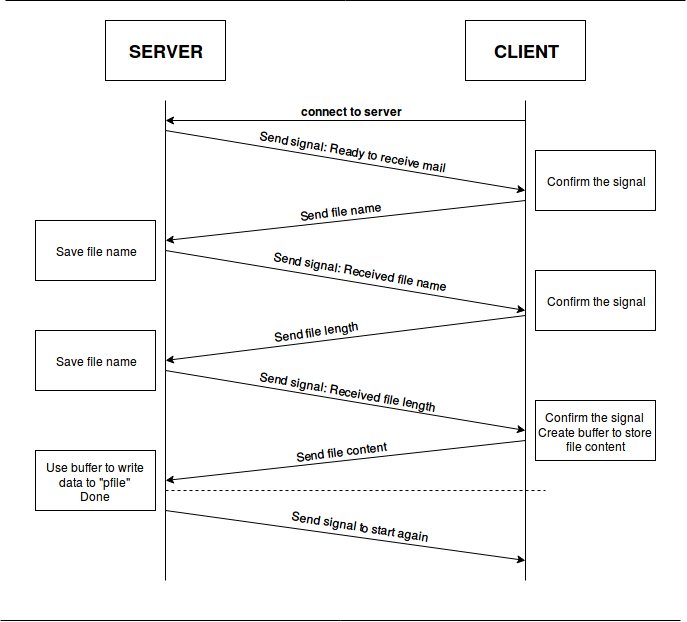
\includegraphics[scale=0.4]{protocol.png}
       \caption{The protocol}
    \end{figure}
  
  \section{Organizing system}
    The system contains one client and one server connecting to each other by using socket. for both client and server, we create a socket first before executing the file transfer. The server then binds to a port and listens to the client's behavior. The client initializes its address then connects to the server. \\
    To transfer file, the server first sends a message to notify that it's ready to receive file. The client confirms the message, request user to input the file's name and send it to server. The server receives it, sends message nofifying that file's name is received. The client then gets the file's length and sends it to the server. The server receives it and sends back a message notifying the file's length received. After confirming that message, the client sends the file's data to the server and waits until the process finished. The server receives it and ask the user to press a button in order to start the process over again.
    \begin{figure}[h]
        \centering
       \includegraphics[height=8.35cm]{server.png}
        \caption{Server}
        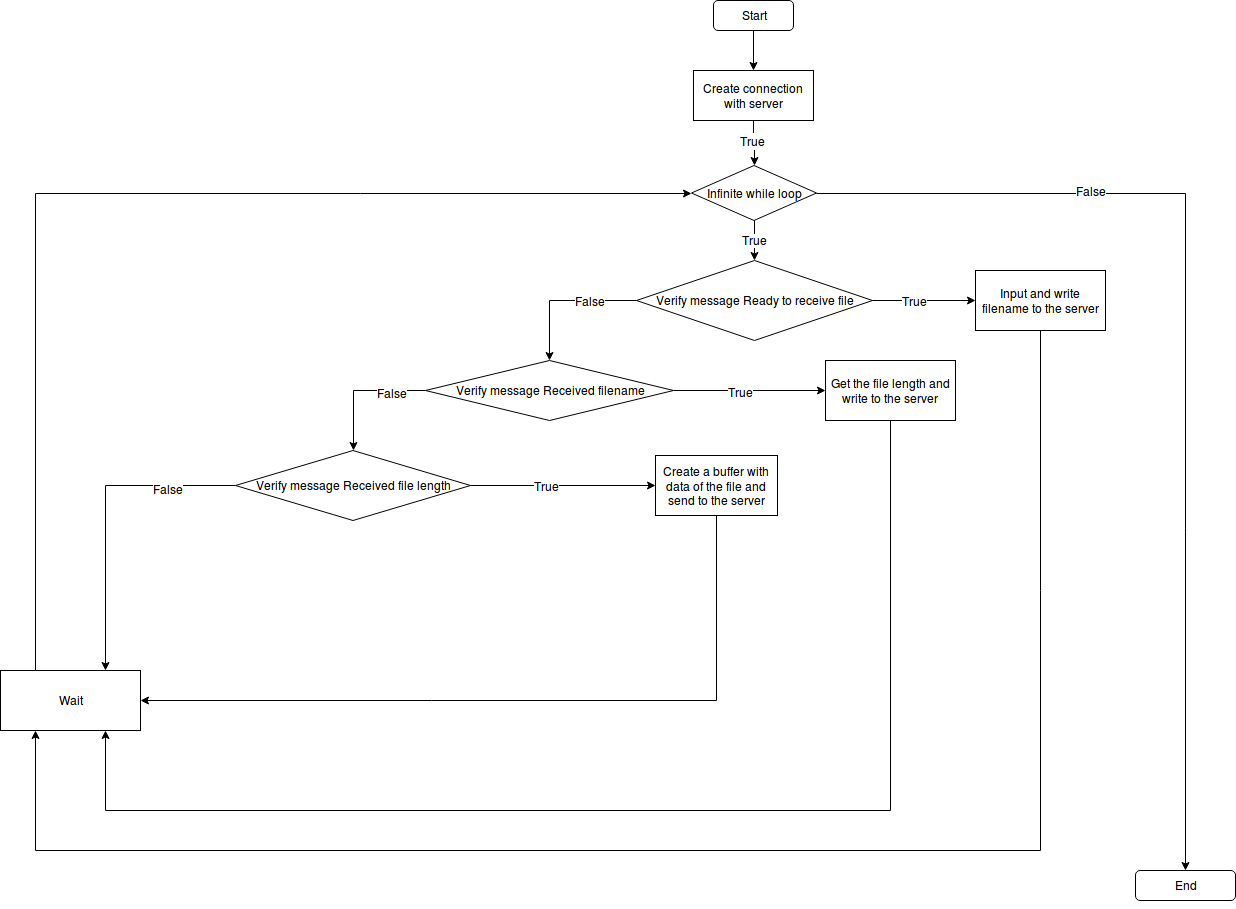
\includegraphics[height=8.35cm]{client.png}
       \caption{Client}
    \end{figure}
    % \begin{figure}[h]
    %  \centering
    %   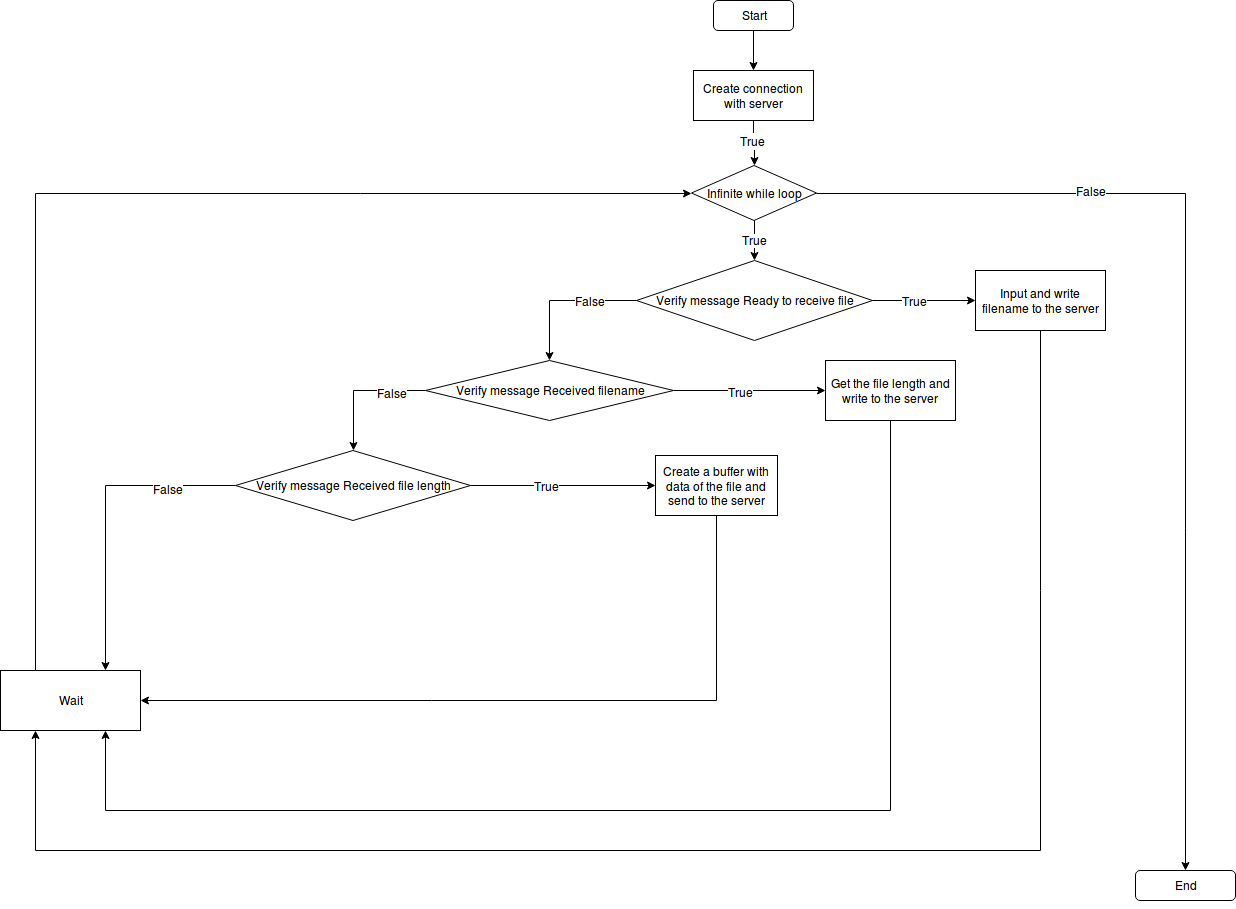
\includegraphics[scale=0.3]{client.png}
    %   \caption{client}
    %     \label{fig:graph2}
    % \end{figure}
 
  \section{Implementing the file transfer}
    The server will response messages which are copied to its array s to the client. The client will read the messages and store it in its array s, then do tasks depend on the strings in that array. To send the file, we first need to send the file name, then the length of it and final is the data.\\
    When the client connects to the server, the server will send "Ready to receive file". The client checks the string using the \textit{strcmp} function and send the name to the server.
    \begin{verbatim}
    if (strcmp(s, "Ready to receive file") == 0)
    {
        // start to send file name to the server
        printf("Ready to receive file\n");
        printf("client> Please enter file name: "); 
        scanf("%s", s);
        pfile = fopen(s, "rb");         
        write(serv, s, strlen(s) + 1);   // send file name to the server
    }
    \end{verbatim}
    Next, the server sends "Received file name" and the client compare again. Now, the file length will be sent.
    \begin{verbatim}
    else if (strcmp(s, "Received file name") == 0)
    {
        // expect to read file length 
        printf("Received file name\n");
        read(cli, s, sizeof(s));
        filelen = atol(s);
        printf("%lu\n", filelen);
        strcpy(s, "Received file length");
        write(cli, s, strlen(s) + 1);
    }
    \end{verbatim}
    Finaly, the client sends the file content by creating a buffer, put everything in it and then send it to the server after receiving "Received file length".
    \begin{verbatim}
    else if (strcmp(s, "Received file length") == 0)
    {
        //  start to send file content to the server 
        printf("Received file length\n");
        // create buffer to send file 
        buffer = (char *)malloc((filelen + 1) * sizeof(char));
        // printf("buffer: %lu\n", sizeof(buffer));
        fread(buffer, filelen, 1, pfile);
        fclose (pfile);
        // send file to the server 
        while(filelen > 0)
        {
            int written = write(serv, buffer, filelen);
            buffer += written;
            filelen -= written;
            // printf("%lu\n", filelen);
        }
    }
    \end{verbatim}
    The server side has a little different. It will check the messages has been sent to the client to know what is expected to be read.\\
    After sending "Ready to receive file", this string will be saved to s and then the server will be ready to receive the file name and create a new file using that name. It also sends "Received file name" to the client at that time.
    \begin{verbatim}
    if (strcmp(s, "Ready to receive file") == 0)
    {
        // expect to read file name from client 
        printf("Ready to receive file\n");
        // numread = read(cli, s, sizeof(s));
        read(cli, s, sizeof(s));
        // printf("numread %d, s = %s\n",numread,s );
        pfile = fopen(s, "wb"); // create a file with the received name 
        strcpy(s, "Received file name"); // send confirming message  
        write(cli, s, strlen(s) + 1);
    }
    \end{verbatim}
    The server then ready to receive the file length
    \begin{verbatim}
    else if (strcmp(s, "Received file name") == 0)
    {
        // expect to read file length 
        printf("Received file name\n");
        read(cli, s, sizeof(s));
        filelen = atol(s);
        printf("%lu\n", filelen);
        strcpy(s, "Received file length");
        write(cli, s, strlen(s) + 1);
    }
    \end{verbatim}
    And finaly prepare for the content of file by again creating a buffer to store what was sent by the client. After that it will write form the buffer a new file in the server side.
    \begin{verbatim}
    else if (strcmp(s, "Received file length") == 0)
    {
        // expect to receive the file content
        printf("Received file length\n");
        // create buffer to receive file
        buffer = (char *)malloc((filelen + 1) * sizeof(char));
        long templen = filelen;
        // read everything in cli to buffer. 
        //This loop is to help reading the whole file
        while (templen > 0)
        {
            int written = read(cli, buffer, templen);
            buffer += written;
            templen -= written;
        }
        // printf("%lu\n", templen);
       // return the buffer pointer to the start of the pointer
        buffer -= filelen; 
        // rewind(buffer);
        while (filelen > 0)
        {
            int written = fwrite(buffer, 1, filelen, pfile);
            buffer += written;
            filelen -= written;
        }
        fclose(pfile);
        strcpy(s, "Done");
        write(cli, s, strlen(s) + 1);
    }
    \end{verbatim}
    \section{Who does what}
    We worked together to find solutions for the labwork. There were some solutions (such as store file length and file content to a buffer and send to server, the server will then determine the file length and file content to create a new file) but we were not able to finish it. Then we choose the best solution (from Hoang Duc Minh) to implement.\\
Hoang Duc Minh coded\\
Le Tan Nhat Linh fixed bug\\
Luong Hung Son, Nguyen Vu Hung, Truong Hai Long wrote the report
\end{document}
